\chapter{Wizualizacja przy pomocy warstw ukrytych sieci VGG-19}
\label{chap:vgg}
\section{Model sieci VGG-19}
\label{vgg-model}

Do bardziej złożonych wizualizacji posłużę się siecią VGG, której architekturę zaprezentowano po raz pierwszy w 2015 roku w publikacji autorstwa Karen Simonyan i 
Andrew Zisserman\cite{vggpaper}. W publikacji zaprezentowano kilka wariantów tej sieci, ja z uwagi na większą ilość warstw użyję wariantu VGG-19.

\begin{figure}[ht]
\centerline{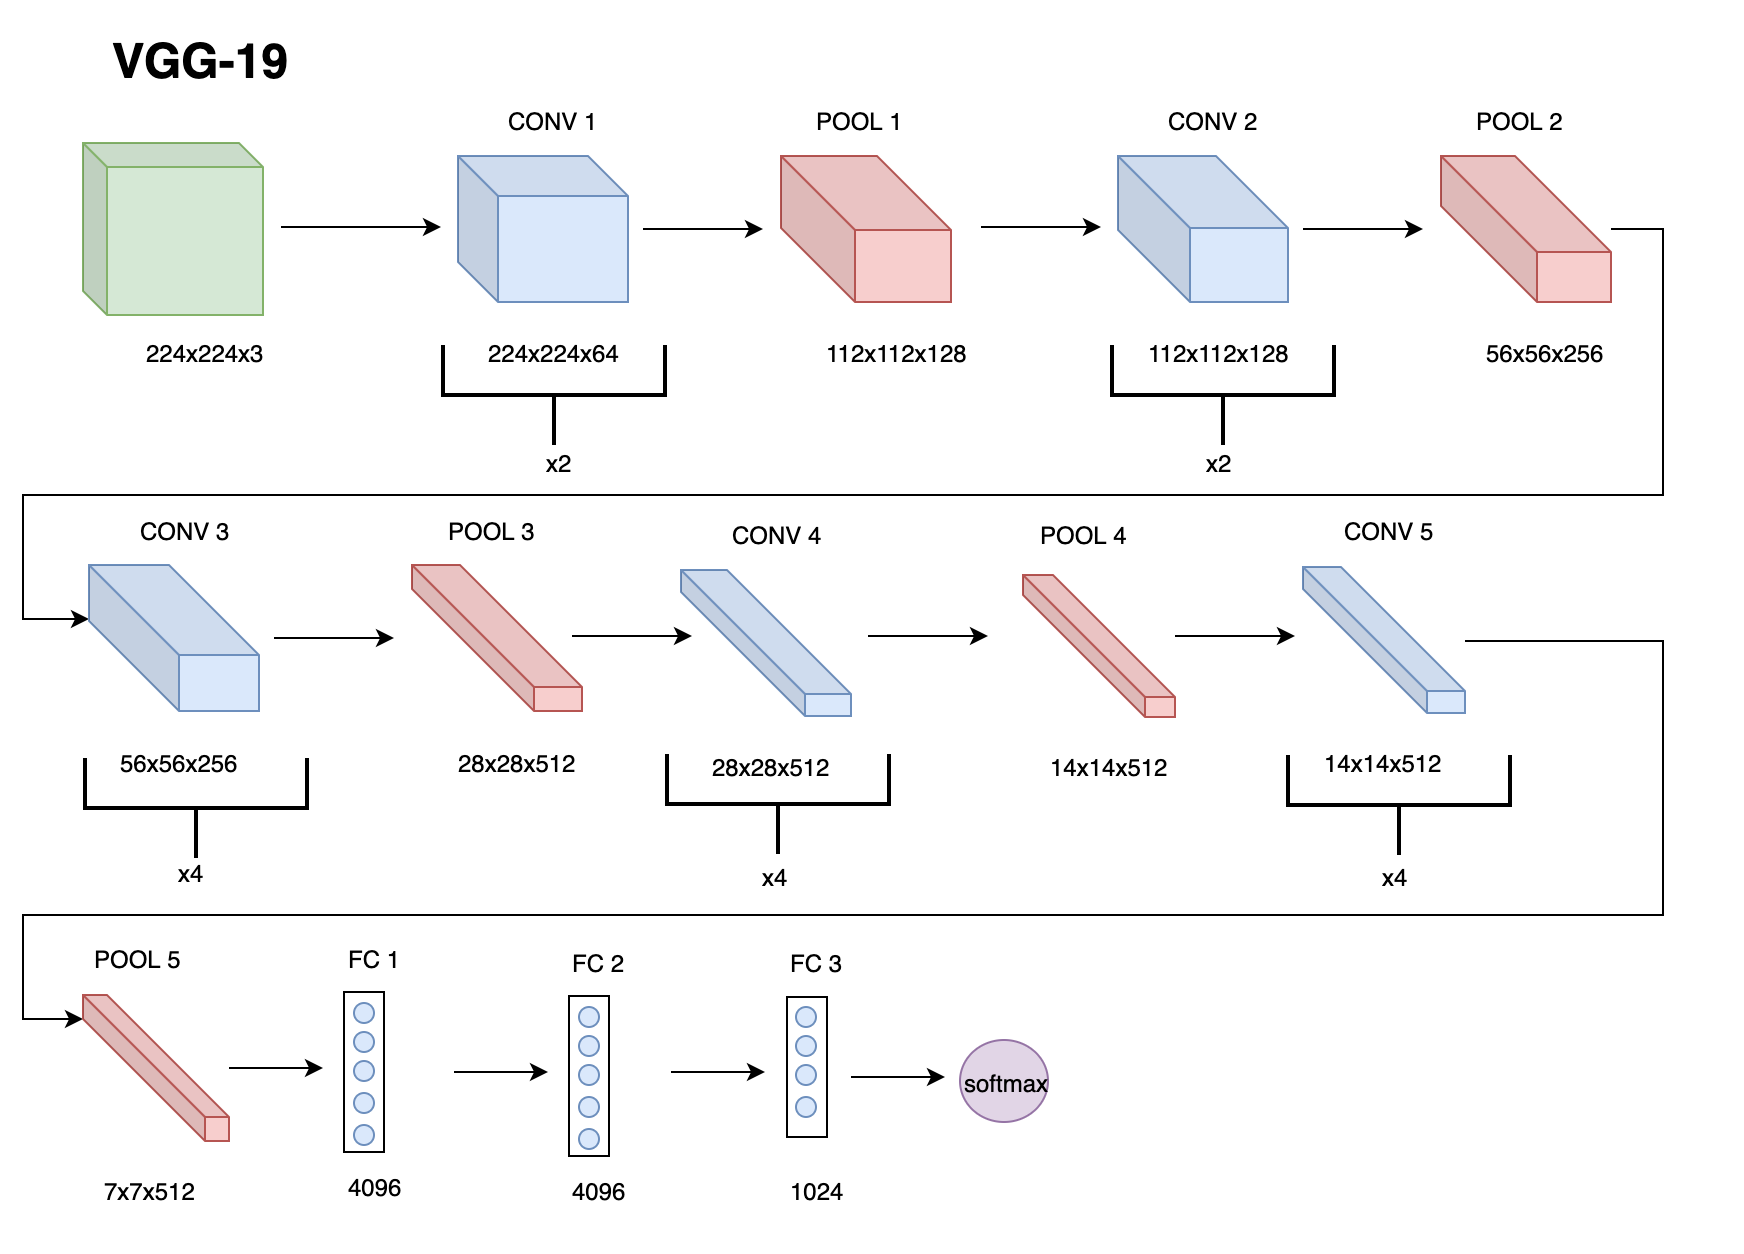
\includegraphics[scale=0.5]{resources/vgg19.png}}
\caption{Schemat modelu sieci VGG-19.}
\label{fig:vgg19-schemat}
\end{figure}

Dopełnienie w przypadku warstw konwolucyjnych wynosi \(p=1\) przy skoku \(s=1\) co sprawia, że warstwy konwolucyjne mogą być ze sobą łączone w łańcuchy niezmieniające wymiarów tensora. W przypadku warstw poolingowych \(p=1\) przy skoku \(s=2\) tym samym, dzielą one dwa pierwsze wymiary przez pół. Sumarycznie daje to 16 warstw możliwych do wykorzystania w wizualizacjach.

\subsection{Wizualizacja sieci VGG poprzez rekonstrukcję obrazu przy pomocy maksymalizacji aktywacji neuronu.}
\label{vgg-mean-activation}

Z racji swoich rozmiarów trening sieci VGG potrafi trwać dniami, nawet przy pomocy GPU. Użyję więc wcześniej wytrenowanej sieci dostępnej bezpośrednio w Kerasie.

\label{lst:vggkeras}
\begin{lstlisting}[language=Python, caption={Wczytywanie wag VGG-19 w Keras.}, captionpos=b]
from keras.applications import VGG19
model = VGG19(include_top=False, weights='imagenet')
\end{lstlisting}

Zastosowane opcje to przedewszystkim zestaw danych na których była trenowana sieć, w tym wypadku zbiór ImageNet\cite{imagenet}, oraz wyłączenie z ładowanego modelu warstw gęstch. Ta ostatnia opcja pozwoli na rekonstukcję obrazu o dowolnej liczbie pikseli (zamiast standardowego dla architektury VGG 224\(\times\)224 pikseli).

Mając załadowany model wraz z wytrenowanymi wagami, wybieram poszczególne filtry z kolejnych warstw konwolucyjnych. Następnie, generuję losowy obrazek o niskiej rozdzielczości, w skali odcieni szarości i wyliczam aktywacje wybranej wcześniej warstwy. Medianę z tych aktywacji traktuję jako wartość mojej funkcji kosztu i modyfikuję wylosowany uprzednio obrazek w celu jej maksymalizacji.
Modyfikacja obrazu polega na dodaniu odpowiednio znormalizowanego gradientu do wartości poszczególnych pikseli. Cały proces treningu składa się z kilkukrotnego skalowania obrazu do wyższych ''rozdzielczości'' i ponawiania procesu optymalizacji. 

Skalowanie jest konieczne ponieważ struktury generowane tą metodą charakteryzują się wysoką częstotliwością (są małe i powtarzalne). Uprzednie wygenerowanie fragmentu wzoru w niskiej rozdzielczości i skalowanie, sprawia, że często wzór jest niejako ''dobudowywany'' zamiast powtarzany - co czasem daje lepsze zrozumienie na co patrzymy, choć nie jest to niestety reguła.

\label{lst:vggmeantraining}
\begin{lstlisting}[language=Python, caption={Wizualizowanie poprzez maksymalizację mediany wybranej warstwy.}, captionpos=b]
output = layers_by_name[layer_name].output
loss = K.mean(output[:, :, :, filter_index])
gradients = K.gradients(loss, input_tensor)[0]
img = generate_grascale_img();
for interpolation_step in image_resize_steps:
    for i in range(EPOCHS_NUMBER):
        loss_val, gradients_val = step([img])
        img += gradients_val 
    resize_img(img);
\end{lstlisting}

Szczegóły takie jak normalizacja gradientu czy konwersja obrazu z postaci nadającej się do treningu na postać zdatną do wyświetlenia zostały pominięte.

\begin{figure}
\subfloat[Wizualizacja filtra nr 5 bloku 1]{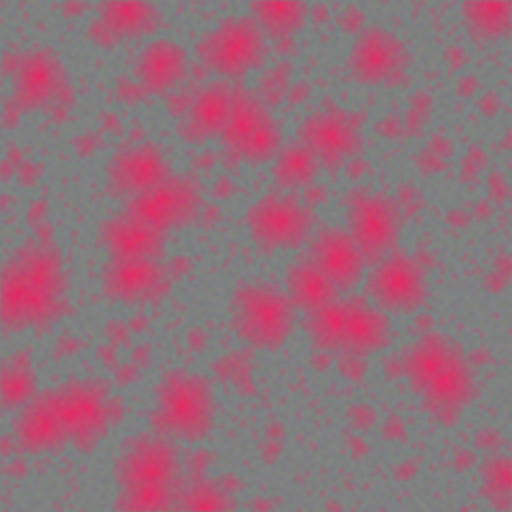
\includegraphics[width = 3in]{resources/vgg_mean_res/block1_conv1_5.png}} 
~
\subfloat[Wizualizacja filtra nr 0 bloku 1]{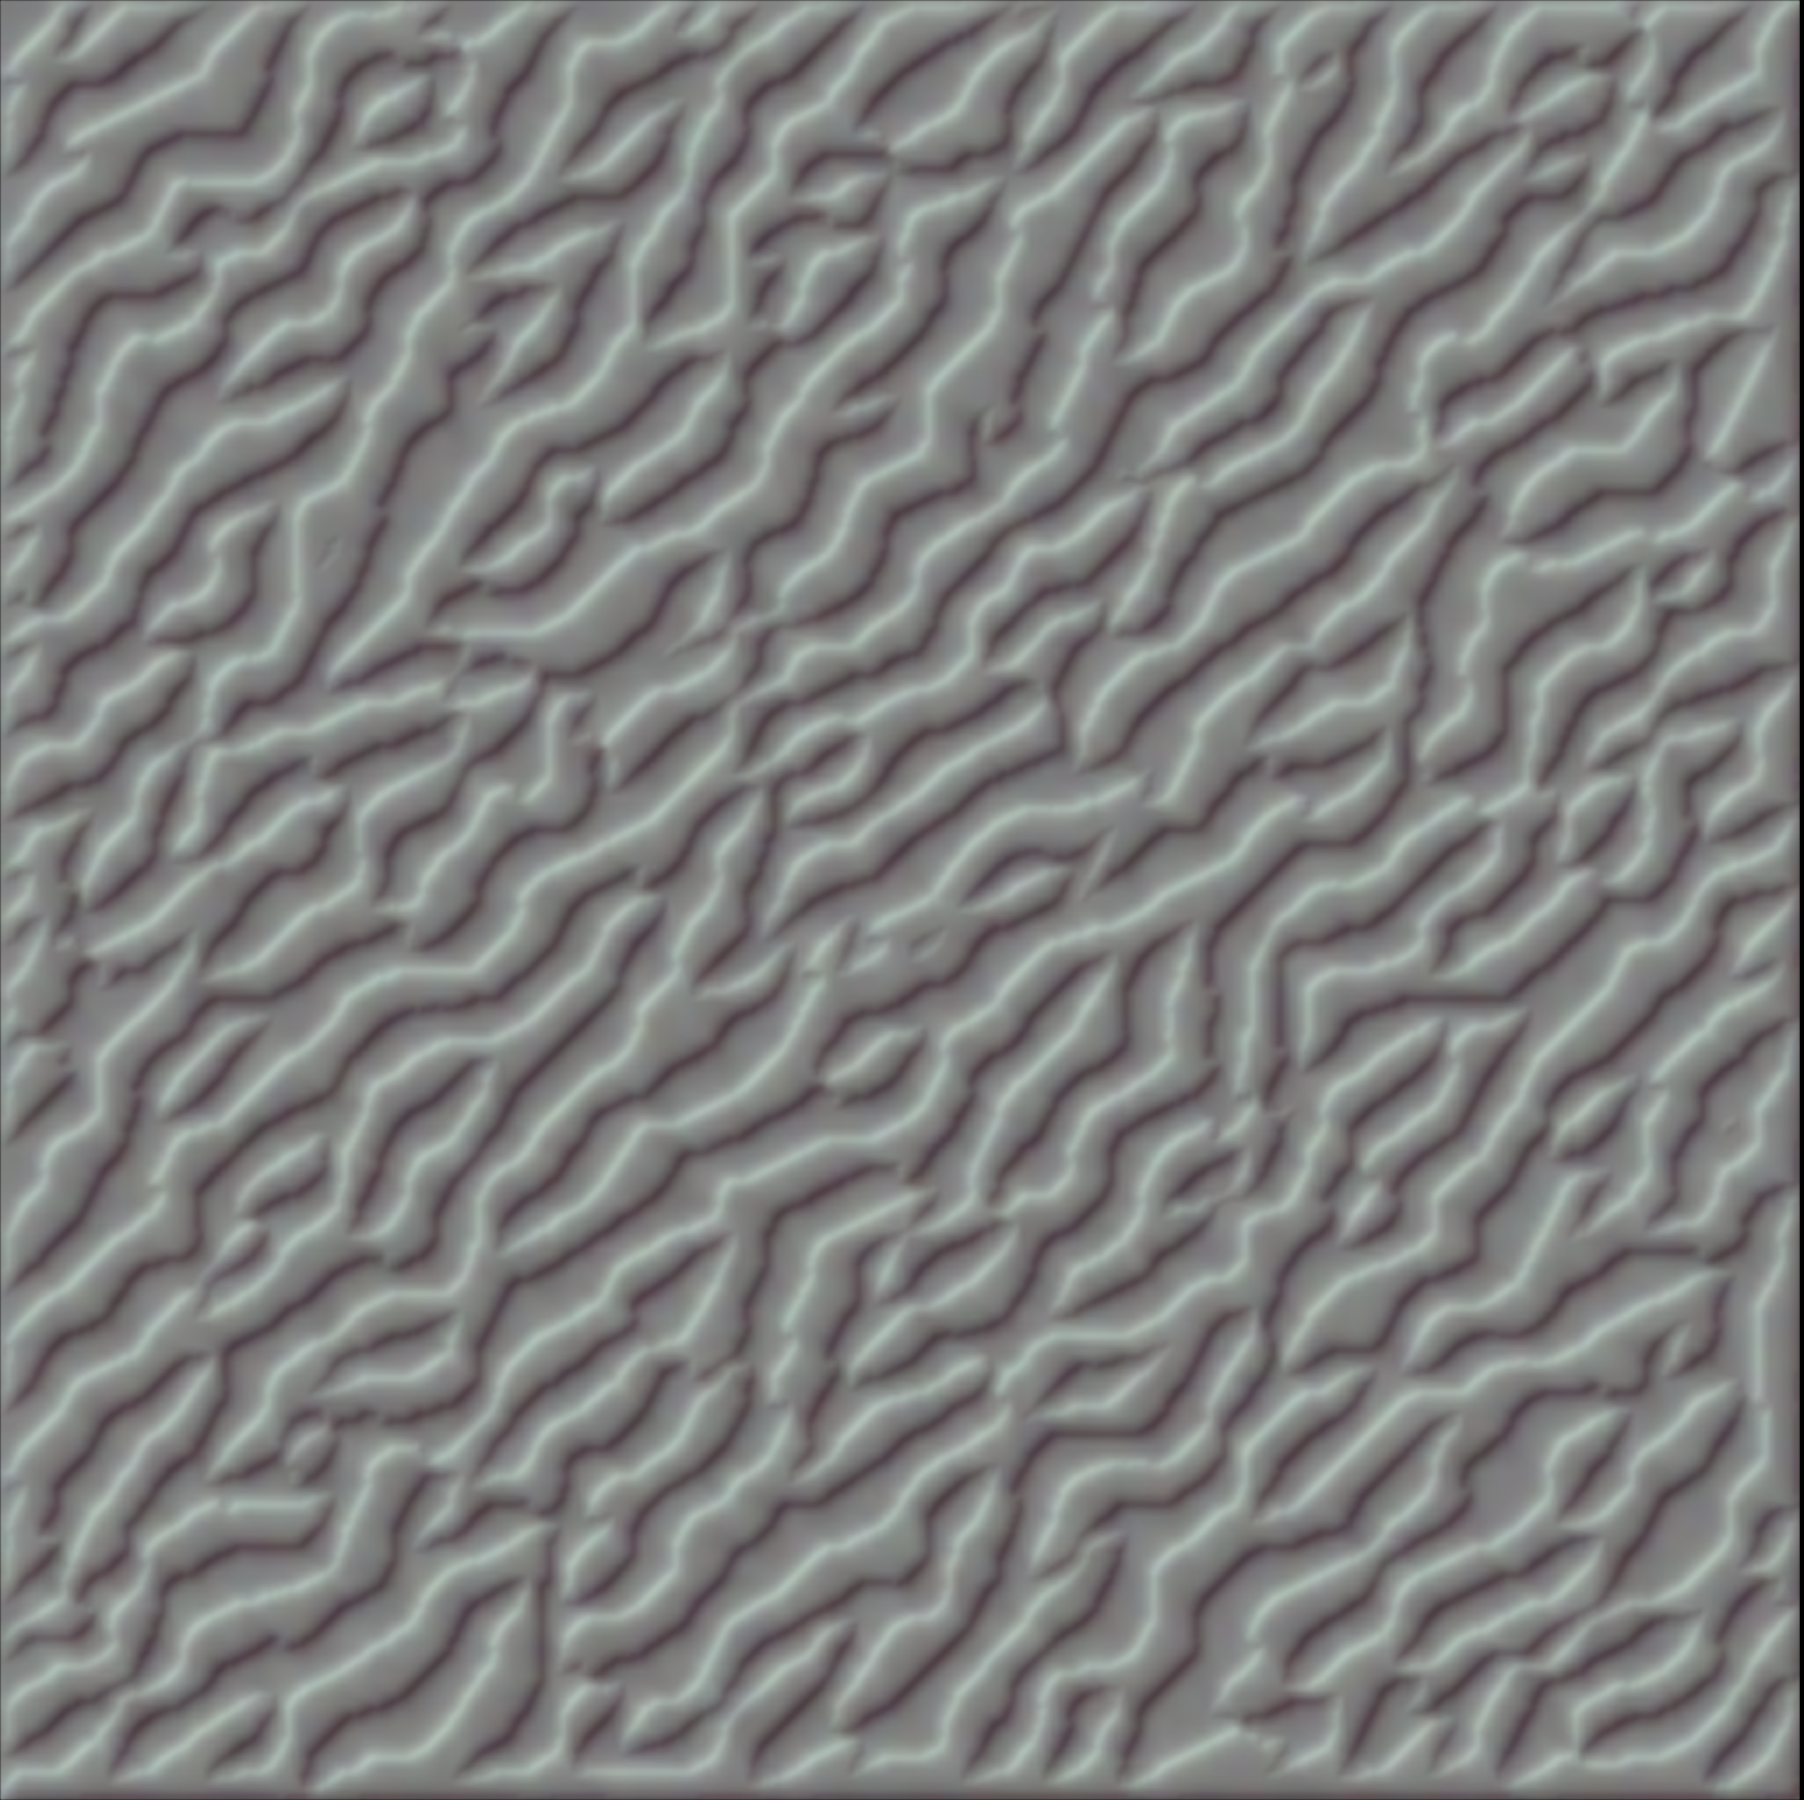
\includegraphics[width = 3in]{resources/vgg_mean_res/vgg_b1c1_0.png}} 
\\
\subfloat[Wizualizacja filtra nr 63 bloku 1]{
\includegraphics[width = 3in]{resources/vgg_mean_res/vgg_b1c1_63.png}} 
~
\subfloat[Wizualizacja filtra nr 33 bloku 2]{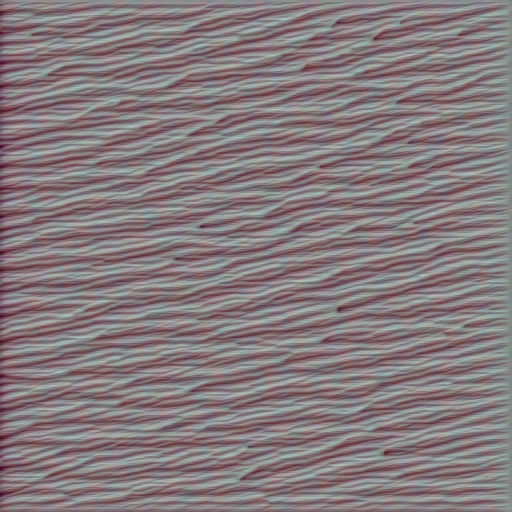
\includegraphics[width = 3in]{resources/vgg_mean_res/block2_conv1_33.png}} 
\caption{Wybrane wizualizacje początkowej warstwy sieci VGG-19 (oznaczonej na rysunku \ref{vgg-model} jako conv1)}
\label{mean-vgg-vis-c1bx}
\end{figure}

\begin{figure}
\subfloat[Wizualizacja filtra nr 120 bloku 2]{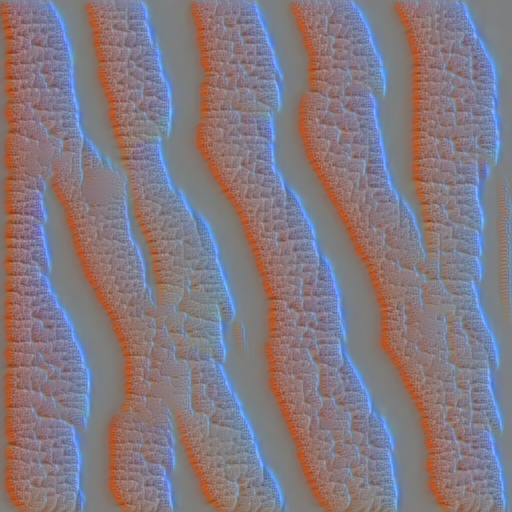
\includegraphics[width = 3in]{resources/vgg_mean_res/block2_conv2_120.png}} 
~
\subfloat[Wizualizacja filtra nr 60 bloku 2]{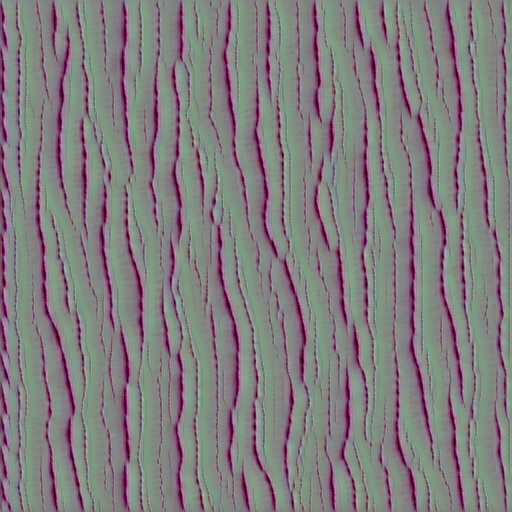
\includegraphics[width = 3in]{resources/vgg_mean_res/block2_conv2_60.png}} 
\\
\subfloat[Wizualizacja filtra nr 80 bloku 2]{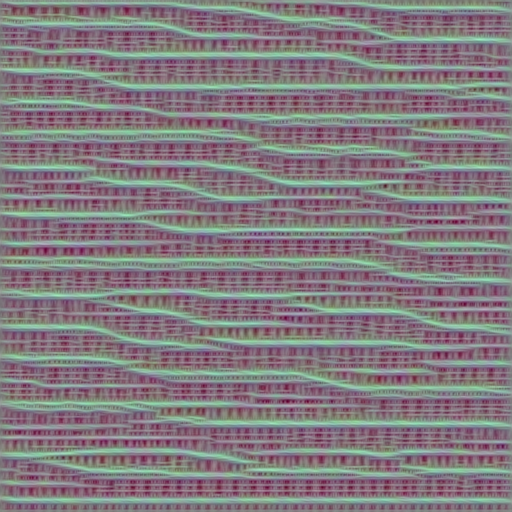
\includegraphics[width = 3in]{resources/vgg_mean_res/block2_conv2_80.png}} 
~
\subfloat[Wizualizacja filtra nr 60 bloku 5]{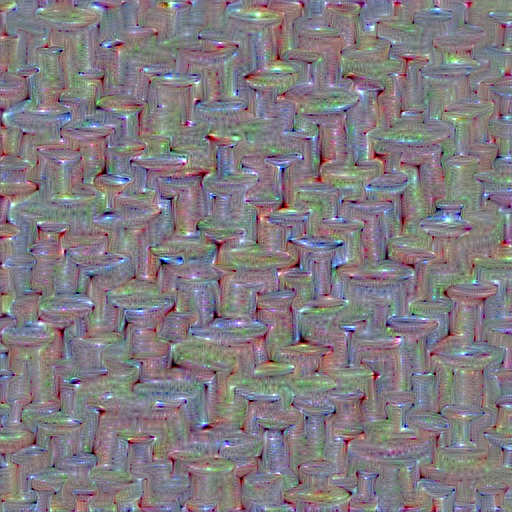
\includegraphics[width = 3in]{resources/vgg_mean_res/block5_conv2_60.png}} 
\caption{Wybrane wizualizacje początkowej warstwy sieci VGG-19 (oznaczonej na rysunku \ref{vgg-model} jako conv1)}
\label{mean-vgg-vis-c1bx}
\end{figure}

